\documentclass[a4paper,10pt]{article}
\usepackage[utf8]{inputenc}
\usepackage[a4paper,
            bindingoffset=0.2in,
            left=1in,
            right=1in,
            top=1in,
            bottom=1in,
            footskip=.25in]{geometry}

%###############################################################################

%\input{~/layout/global_layout}


%###############################################################################

% packages begin

\usepackage[
  backend=biber,
  sortcites=true,
  style=alphabetic,
  eprint=true,
  backref=true
]{biblatex}
\addbibresource{bibliographie.bib}
\usepackage[acronym]{glossaries}

\usepackage{euscript}[mathcal]
% e.g. \mathcal{A} for fancy letters in mathmode
\usepackage{amsmath,amssymb,amstext,amsthm}

\usepackage{mdframed}
\newmdtheoremenv[nobreak=true]{problem}{Problem}[subsection]
\newmdtheoremenv[nobreak=true]{claim}{Claim}[subsection]
\newtheorem{definition}{Definition}[subsection]
\newtheorem{lemma}{Lemma}[claim]
\newtheorem{plemma}{Lemma}[problem]

\usepackage{mathtools}
\DeclarePairedDelimiter\ceil{\lceil}{\rceil}
\DeclarePairedDelimiter\floor{\lfloor}{\rfloor}

\usepackage{enumerate}
\usepackage[pdftex]{graphicx}
\usepackage{subcaption}
% 'draft' für schnelleres rendern mitübergeben -> [pdftex, draft]
% dadruch wird nicht das bild mitgerendered, sondern nur ein kasten mit bildname -> schont ressourcen

\usepackage{hyperref}

\usepackage{tikz}
\usetikzlibrary{arrows,automata,matrix,positioning,shapes}

% for adding non-formatted text to include source-code
\usepackage{listings}
\lstset{language=Python,basicstyle=\footnotesize}
% z.B.:
% \lstinputlisting{source_filename.py}
% \lstinputlisting[lanugage=Python, firstline=37, lastline=45]{source_filename.py}
%
% oder
%
% \begin{lstlisting}[frame=single]
% CODE HERE
%\end{lstlisting}
\usepackage{algorithm}
\usepackage{algpseudocode}

\usepackage{wasysym}

\usepackage{titling}
\usepackage{titlesec}
\usepackage[nocheck]{fancyhdr}
\usepackage{lastpage}
\usepackage{csvsimple}

\usepackage{kantlipsum}
\usepackage[colorinlistoftodos,prependcaption,textsize=tiny]{todonotes}

% packages end
%###############################################################################

\pretitle{% add some rules
  \begin{center}
    \LARGE\bfseries
} %, make the fonts bigger, make the title (only) bold
\posttitle{%
  \end{center}%
  %\vskip .75em plus .25em minus .25em% increase the vertical spacing a bit, make this particular glue stretchier
}
\predate{%
  \begin{center}
    \normalsize
}
\postdate{%
  \end{center}%
}

\titleformat*{\section}{\Large\bfseries}
\titleformat*{\subsection}{\large\bfseries}
\titleformat*{\subsubsection}{\normalsize\bfseries}

\titleformat*{\paragraph}{\Large\bfseries}
\titleformat*{\subparagraph}{\large\bfseries}

%###############################################################################

\pagestyle{fancy}
\fancyhf{}
% l=left, c=center, r=right; e=even_pagenumber, o=odd_pagenumber; h=header, f=footer
% example: [lh] -> left header, [lof,ref] -> fotter left when odd, right when even
%\fancyhf[lh]{}
%\fancyhf[ch]{}
%\fancyhf[rh]{}
%\fancyhf[lf]{}
\fancyhf[cf]{\footnotesize Page \thepage\ of \pageref*{LastPage}}
%\fancyhf[rf]{}
\renewcommand{\headrule}{} % removes horizontal header line

% Fotter options for first page

\fancypagestyle{firstpagestyle}{
  \renewcommand{\thedate}{\textmd{}} % removes horizontal header line
  \fancyhf{}
  \fancyhf[lh]{\ttfamily M.Sc. Computer Science\\KTH Royal Institute of Technology}
  \fancyhf[rh]{\ttfamily Period 4\\\today}
  \fancyfoot[C]{\footnotesize Page \thepage\ of \pageref*{LastPage}}
  \renewcommand{\headrule}{} % removes horizontal header line
}
%###############################################################################

\newcommand\extrafootertext[1]{%
    \bgroup
    \renewcommand\thefootnote{\fnsymbol{footnote}}%
    \renewcommand\thempfootnote{\fnsymbol{mpfootnote}}%
    \footnotetext[0]{#1}%
    \egroup
}

%###############################################################################

\title{
  \normalsize{DD2356 VT25 Methods in}\\
  \normalsize{High Performance Computing}\\
  \large{Assignment 1}
}
\author{
  \small Rishi Vijayvargiya\textsuperscript{\textdagger}\\[-0.75ex]
%  \footnotesize\texttt{MN: }\\[-1ex]
  \scriptsize\texttt{rishiv@kth.se}
  \and
  \small Paul Mayer\textsuperscript{\textdagger}\\[-0.75ex]
%  \footnotesize\texttt{MN: }\\[-1ex]
  \scriptsize\texttt{pmayer@kth.se}
  \and
  \small Lennard Herud\textsuperscript{\textdagger}\\[-0.75ex]
%  \footnotesize\texttt{MN: }\\[-1ex]
  \scriptsize\texttt{herud@kth.se}
}
\date{}

%###############################################################################
% define Commands

\newcommand{\N}{\mathbb{N}}
\newcommand{\R}{\mathbb{R}}
\newcommand{\Z}{\mathbb{Z}}
\newcommand{\I}{\mathbb{I}}

\newcommand{\E}{\mathbb{E}}
\newcommand{\Prob}{\mathbb{P}}

\renewcommand{\epsilon}{\varepsilon}

%###############################################################################
\makeatletter
\renewcommand*{\@fnsymbol}[1]{\ensuremath{\ifcase#1\or \dagger\or \ddagger\or
   \mathsection\or \mathparagraph\or \|\or **\or \dagger\dagger
   \or \ddagger\ddagger \else\@ctrerr\fi}}
\makeatother
%###############################################################################

\begin{document}
\maketitle
\extrafootertext{\textsuperscript{\textdagger}Authors made equal contribution to the assignment}
\thispagestyle{firstpagestyle}

% \listoftodos
\vspace{1em}

% content begin
%

\section*{Prefix}
The code and other utilities associated with for our assignment can be found at this location: \url{https://github.com/paulmyr/DD2356-MethodsHPC/tree/master/1_dardel_simple_benchmarking}.

% \tableofcontents
% \newpage

\section{Compiling and Running on Dardel}
The steps for running the program first required us to login to Dardel and compile the program. Then, we executed different commands based on the requirement to run in interactive or batch mode. 

\subsection{Logging in to Dardel and Compiling}
Logging in to Dardel can be doen using Kerberos, as described \href{https://support.pdc.kth.se/doc/login/mac_login/}{here} (under the \textit{Own Mac OS X} section). The compilation can be done using the \verb|cc| command. To summarize: 
\begin{itemize}
\item Obtain kerberos ticket using: \verb|/usr/bin/kinit username@NADA.KTH.SE|
\item SSH to Dardel: \verb|ssh -o GSSAPIAuthentication=yes  username@dardel.pdc.kth.se|
\item Add the required code to a file, for ex: \verb|mpi_hello_world.c| 
\item Compile the file with the \verb|cc| command: \verb|cc mpi_hello_world.c -o mpi_hello_world.out|
\end{itemize}

Next steps depend on whether we want the task to be run in interactive mode or batch mode. 

\subsection{Batch Mode}
\begin{itemize}
\item Create a job-script: For our program, this is the \verb|run_mpi_hello_world.sh| file in the repository, present \href{https://github.com/paulmyr/DD2356-MethodsHPC/blob/master/1_dardel_simple_benchmarking/code/run_mpi_hello_world.sh}{here}.
\item Submit the job: This is done using the command \verb|sbatch ./run_mpi_hello_world.sh|
\item Eventually, the job was executed. We redirected the output to a \verb|log_dd2356_e1| file. The file with the output can be found \href{https://github.com/paulmyr/DD2356-MethodsHPC/blob/master/1_dardel_simple_benchmarking/code/log_dd2356_e1}{here} in the repo.
\end{itemize}

\subsection{Interactive Mode}
\begin{itemize}
\item Request for job allocation using \verb|salloc|. We ran the command with the following arguments: \\ {\small \verb|salloc -t 00:30:00 --nodes 1 --ntasks-per-node 128 --cpus-per-task 1 -A edu25.DD2356 -p shared|}
\item Launch program using \verb|srun| on the allocated node: \\ \verb|srun -n 128 ./mpi_hello_world.out > log_dd2356_e1_i|. \\ The output produced can be found in the \verb|log_dd2356_e1_i| file \href{https://github.com/paulmyr/DD2356-MethodsHPC/blob/master/1_dardel_simple_benchmarking/code/log_dd2356_e1_i}{here} in the repository. 
\item Once our execution is done, we can relinquish the allocated node by using \verb|exit|.  
\end{itemize}


% \verb|salloc -t 00:30:00 --nodes 1 --ntasks-per-node 128 --cpus-per-task 1 -A edu25.DD2356 -p shared|
% \verb|srun -n 128 ./mpi_hello_world.out > log_dd2356_e1_i|

\section{Sustainability and Supercomputers}
  Following the assumption of the previous task, that Dardel uses AMD EPYC™ 7742 cpus, we get a Thermal Design Power (TDP) of $ 225 W $ as stated in \url{https://www.topcpu.net/de/cpu/amd-epyc-7742}.
  Using the \verb|Green algorithm calculator| (\url{https://calculator.green-algorithms.org/}) we can calculate the CO2equivalents of running an algorithm for 12 hours on 10 Dardel computing nodes only utilizing CPU processing power.
  Each node uses two 64 core processors. The memory differs per node, we assume using the most commonly \verb|NAISS thin node| with $256GB $ of memory per node as stated in \url{https://www.pdc.kth.se/hpc-services/computing-systems/dardel-hpc-system/about-the-dardel-system-1.1053338}.
  So our algorithm inputs result in the following values:
  \begin{itemize}
    \item Runtime: 12hrs,
    \item Type of cores: CPU,
    \item Number of cores: 1280 $10 nodes*2 cpus/node*64cores/cpu$, 
    \item TDP: $225 W$,
    \item Memory $ 640 GB = 64GB/node * 10 nodes$
  \end{itemize}

  The output retrieved can be seen in a tabular format at \href{https://github.com/paulmyr/DD2356-MethodsHPC/blob/master/1_dardel_simple_benchmarking/misc/GreenAlgorithms_results_tabular.txt}{this} location in the repository.
  The power consumption equals $5.4 MWh$ and the carbon footprint of the job is 30.59 kg CO2 equivalents,
  for the HPC located in Sweden, which underlines the need for sustainable usage of HPC ressources.

  Since these results are relatively high, we assume the TDP is given per chip, but used as TDP/core by the algorithm. We adapt our inputs by $225W/64cores = 3.515625 W/core$.
  
  With the adapted TDP, we get the output that can be seen in tabular format at \href{https://github.com/paulmyr/DD2356-MethodsHPC/blob/master/1_dardel_simple_benchmarking/misc/GreenAlgorithms_results_TDP_tabular.txt}{this} location in the repository.
  The power consumption equals now $88.7 kWh$ and the carbon footprint of the job is 502.95 g CO2 equivalents,
  for the HPC located in Sweden, which is closer to the results shown in the lecture and more reasonable w.r.t. power dimensioning on the Dardel cluster.

\section{The Memory Mountain}
  We ran the script on dardel.
  We inquired that dardel uses the AMD EPYC™ 7742 cpus.
  This implies the following cache sizes:
  \begin{itemize}
  \item L1: 96 KB(per core), 
  \item L2: 512 KB(per core),
  \item L3: 256 MB(shared)
  \end{itemize}
  The results\footnote{Results found \href{https://github.com/paulmyr/DD2356-MethodsHPC/blob/master/1\_dardel\_simple\_benchmarking/misc/results.txt}{here}.} are visualised in Figure \ref{fig:mem_mountain}.
  \begin{figure}[H]
    \centering
    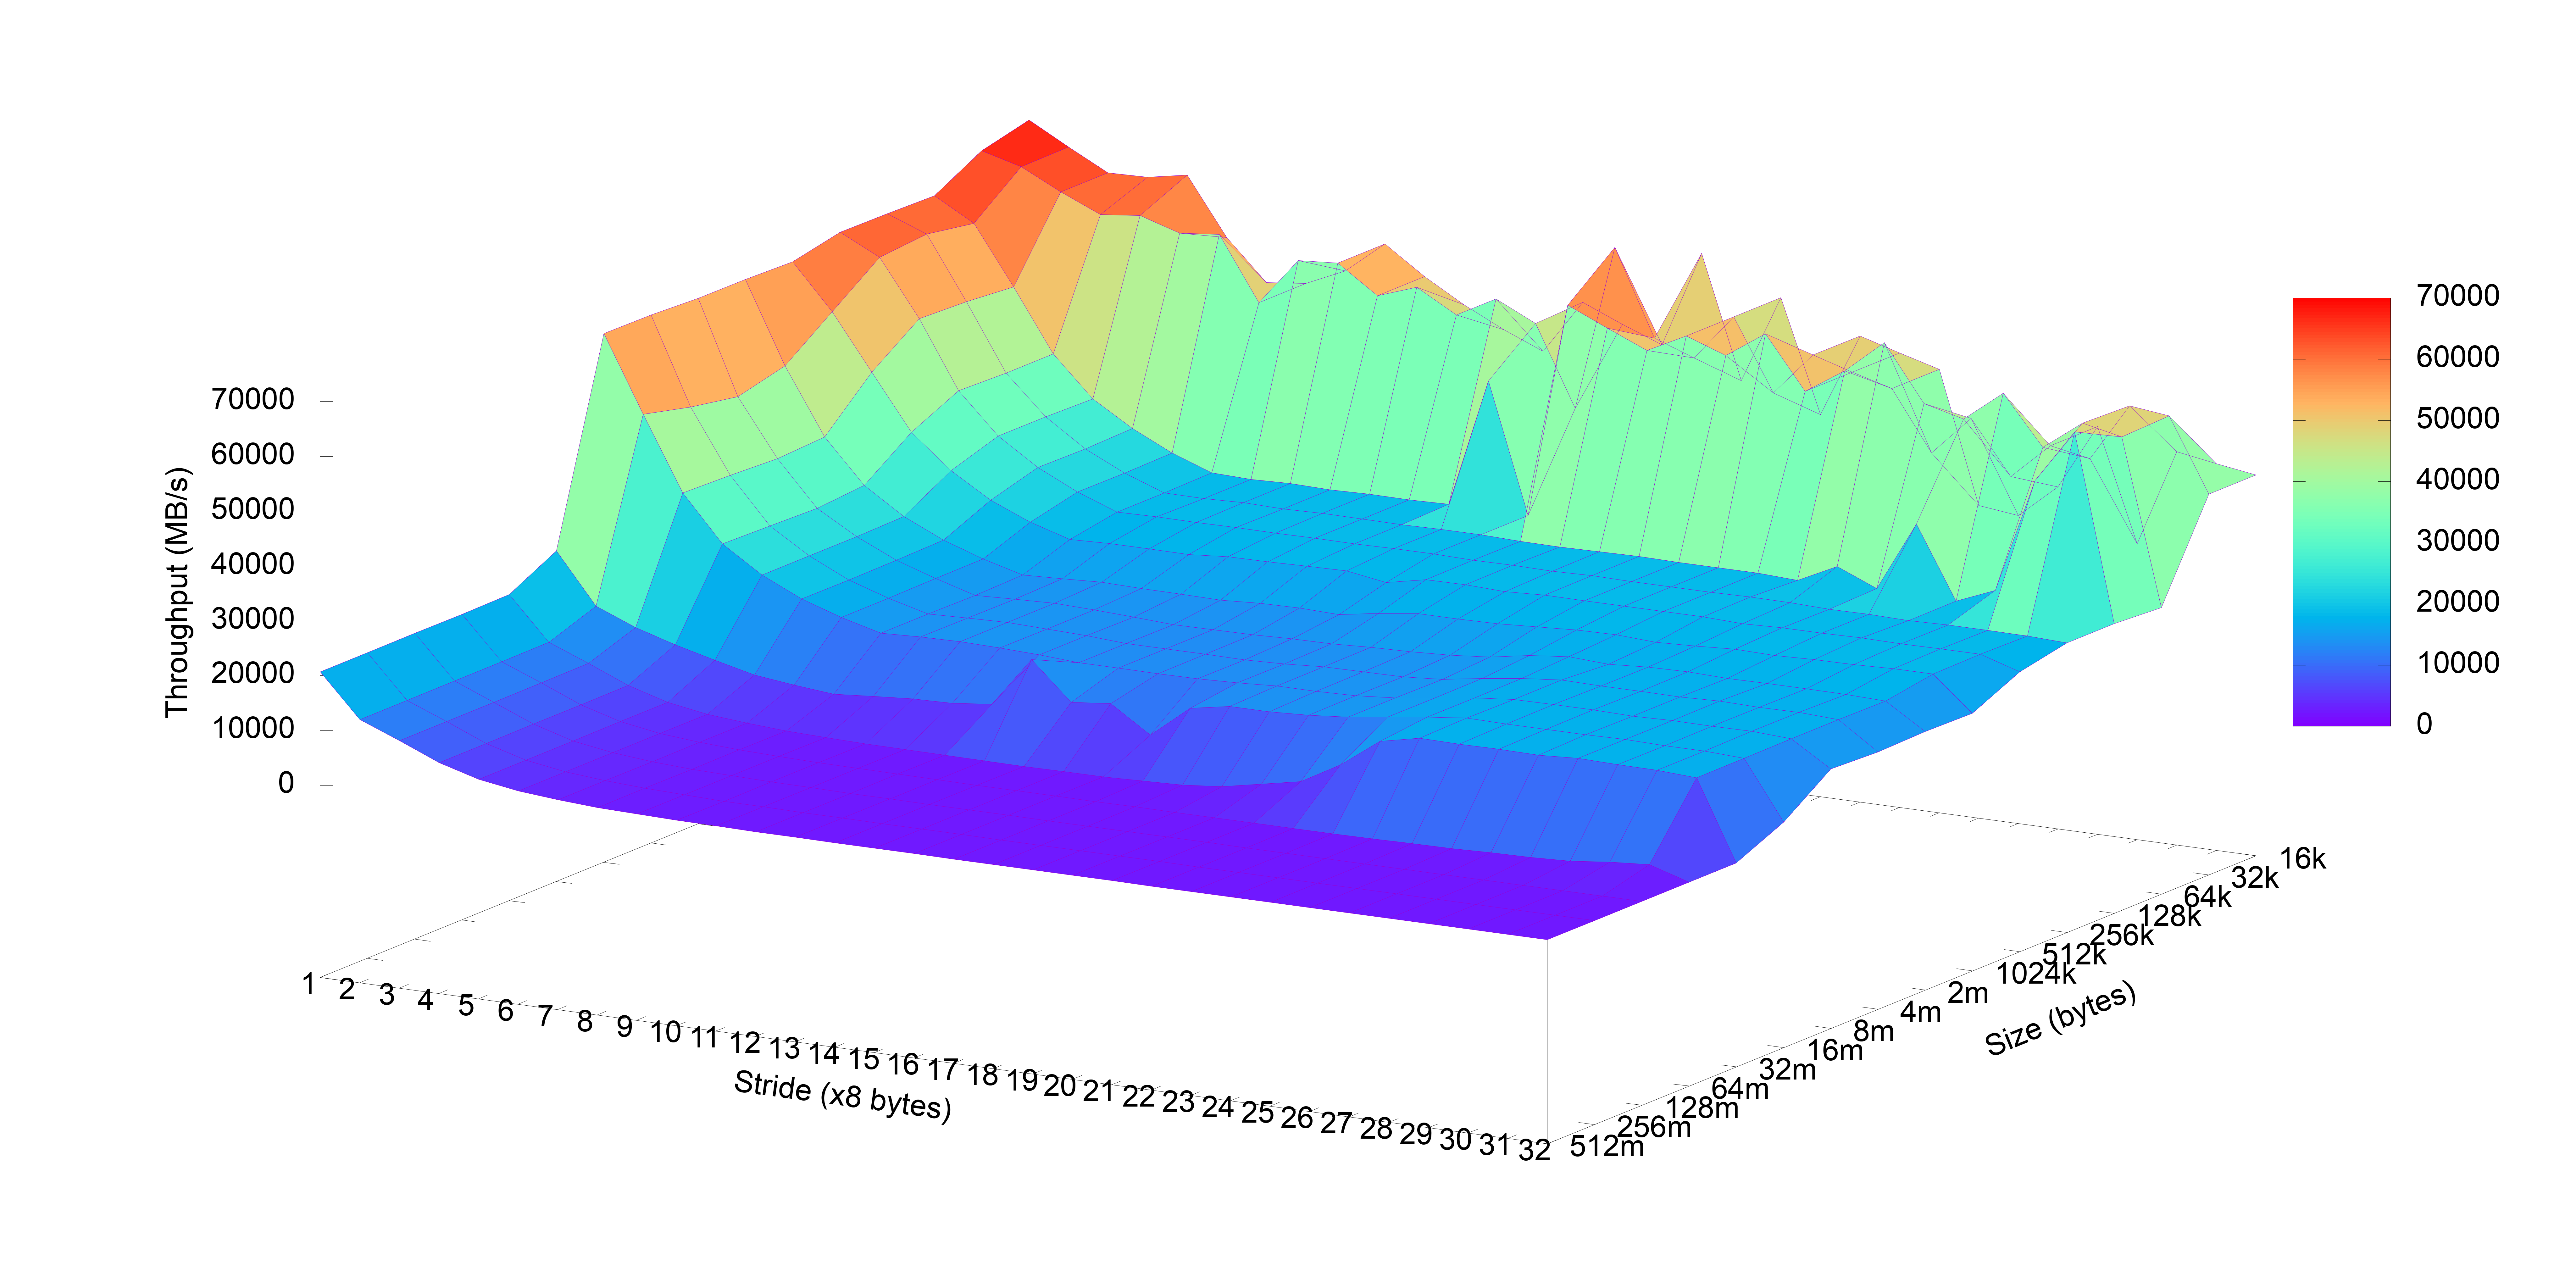
\includegraphics[width=0.9\textwidth]{images/memory_mountain}
    \caption{Memory Mountain Plot}
    \label{fig:mem_mountain}
  \end{figure}
  It clearly shows that the smaller stride and array sizes are, the higher the throughput.
  Inversly the same holds true.
  The bigger the strides and array sizes are, the worse the throughput becomes.
  Suprisingly, for big array sizes (e.g. 512 MB), a stride size of 1 still produces high throughput, even tho the array size surpasses the L3 cache size.

  This has to do with prefetching.
  Prefetching refers to the technique of fetching data that might be used in the near future based in faster memory before it is actually used for the computation.
  This greatly increases performance mainly because fetching data from memory is magnitudes slower than performing arithmetic operations in the processing unit.
  The cpu tries to pre fetch data based on spatial locality, meaning data stored close to the referenced data.
  Spatial Locality means that all those instructions that are stored nearby to the recently executed instruction have a high chance of execution
  It refers to the use of data elements(instructions) that are relatively close in storage locations.
  Spatial locality describes that there is an increased likelyhood that data stored spatially close to recently fetched data is referenced in the near future.
  Many computations perform computations on Lists, Fields or Meshes.
  This means that computations have to be performed on multiple elements typically stored close to each other.
  That is the main reason why increasing the stride reduces spatial locality.
  All of a sudden, elements that are not stored together need to be fetched after each other.
  With a stride size of 1 however, the cpu is able to guess corretly with very high probability, boosting the performance even tho the array size increases the L3 cache size.

  Temporal locality on the other hand describes that data stored at a certain location has an increased likelyhood of beeing fetched again after having been referenced once.
  The main reason for this is that most of heavy computations perform operations in loops, and most of the times is performed on the same data (or data stored in the same location).
  This especially holds true if the data is within a small multiple of the cache size.
  However, for very large data arrays, it might take multiple fetching cylces until the same data location is referenced again, therefore will decrease the temperal locality.
 % content end
 %###############################################################################
 
 % \printbibliography
 
 \end{document}
